\documentclass{report}

\input{../preamble}
\input{../macros}
\input{../letterfonts}


\begin{document}

\newpage% or \cleardoublepage
% \pdfbookmark[<level>]{<title>}{<dest>}
\pdfbookmark[section]{\contentsname}{toc}

\pagebreak

\section{Global Min-Cut}
We start by stating the question we are trying to solve.
\qs{Global Min-Cut Problem}{
    We are given an unweighted and undirected graph $G = (V, E)$. A ``cut'' of the graph is a partition of the vertices into two sets such that each set is non-empty. The ``cost'' of the cut (also called the cut ``size'') is the number of edges that have one endpoint in each set. The goal is to find the cut with the smallest cost.
}

\noindent Let $n:= |V|$. We consider two randomized algorithms:
\begin{itemize}
    \item Karger's Algorithm (1995) - poly$(n)$-time.
    \item Karger-Stein Algorithm (1996) - $\tilde{O}(n^2)$ time.
\end{itemize}

\subsection{Edge Contraction}
The key idea in both algorithms is edge contraction. Given an edge $(u, v)$, we can contract it by removing the edge and merging the two vertices into a single vertex. The new vertex will have all the edges that $u$ and $v$ had. For example:

\begin{center}
    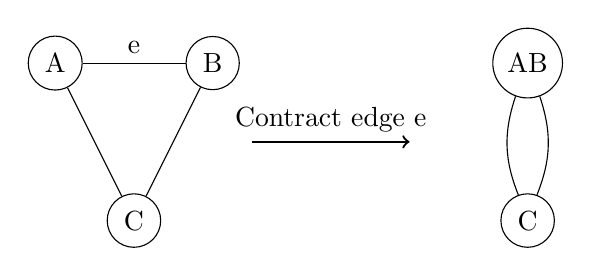
\begin{tikzpicture}
        \node[draw, circle] (A) at (0, 1) {A};
        \node[draw, circle] (B) at (2, 1) {B};
        \node[draw, circle] (C) at (1, -1) {C};
    
        \draw (A) -- (B) node[midway, above] {e};
        \draw (B) -- (C);
        \draw (A) -- (C);
    
        \draw[->, thick] (2.5, 0) -- (4.5, 0) node[midway, above] {Contract edge e};
    
        \node[draw, circle] (AB) at (6, 1) {AB};
        \node[draw, circle] (C2) at (6, -1) {C};

        \draw (AB) to [bend left=20] (C2);
        \draw (AB) to [bend right=20] (C2);
    \end{tikzpicture}
\end{center}
\noindent Each contraction reduces the number of vertices by 1, and we want to stop when we have two vertices left. This leaves us with two vertices and many edges between them.
\nt{We allow multi-edges.}
\noindent \textbf{Question:} Should we keep self-edges?

\noindent \textbf{Answer:} No. Delete them.

\noindent The observation we make is that we win iff edges at the end are a min-cut.

\subsection{Karger's Algorithm}
\noindent The algorithm is as follows:
\begin{itemize}
    \item Randomly pick an edge $(u, v)$.
    \item Contract $(u, v)$.
    \item Repeat until 2 vertices are left.
\end{itemize}
\mlenma{}{For any min-cut C, the probability that Karger's algorithm finds C is $\geq \frac{1}{\text{poly}(n)}$.}
\begin{proof}
    Let $e_1, e_2, \ldots$ be the edges we contract. Let's start by considering $P(e_1 \in C)$.

    We first have $P(e_1 \in C) = \frac{|C|}{|E|}$, but there's something better to notice. Let $d$ be the minimum degree of any vertex in $G$. Then $|C| \leq d$ and $|E| \geq \frac{dn}{2}$. So $P(e_1 \in C) \leq \frac{2}{n}$ and $P(e_1 \notin C) \geq 1 - \frac{2}{n}$.

    Now consider $P(e_2 \notin C \mid e_1 \notin C)$. By the same analysis, we have $P(e_2 \notin C \mid e_1 \notin C) \geq 1- \frac{2}{n-1}$. This is because after we contract $e_1$, we have $n-1$ vertices left. So, $C$ is still a min-cut with respect to the remaining vertices. Set $d$ as the new minimum degree, and we have $|C| \leq d$ and $|\text{remaining edges}| \geq \frac{d(n-1)}{2}$. Then:
    \begin{align*}
        P(e_2 \in C \mid e_1 \notin C) = \frac{|C|}{|\text{remaining edges}|} \leq \frac{d}{\frac{d(n-1)}{2}} = \frac{2}{n-1}.
    \end{align*}
    Now:
    \begin{align*}
        P(e_3 \notin C | e_1, e_2 \notin C) &\geq 1 - \frac{2}{n-2} \\
        &\vdots \\
        P(e_k \notin C | e_1, \ldots, e_{k-1} \notin C) &\geq 1 - \frac{2}{n-k+1}.
    \end{align*}
    So,
    \begin{align*}
        P(\text{we find } C) = P(e_1, \ldots, e_{n-2} \notin C) &\geq \left(\frac{n-2}{n}\right) \left(\frac{n-3}{n-1}\right) \ldots \left(\frac{1}{3}\right) \\
        &\approx \frac{2}{n(n-1)}.
    \end{align*}
\end{proof}
\textbf{Conclusion:} The algorithm succeeds with probability $\geq  \frac{2}{n(n-1)}$.

\noindent \textbf{New Goal:} Find min-cut with $\geq 1 - \frac{1}{n^2}$ probability. 

\noindent \textbf{Idea:} Repeat $t$ times and return the best cut we find. (We will determine the value for $t$ below.)

The probability that all $t$ trials fail is $\leq \left(1 - \frac{2}{n(n-1)}\right)^t$. We want this to be $\leq \frac{1}{n^2}$. We utilize the inequality below:
\begin{align*}
    \left(1 - \frac 1k\right)^k \leq \frac 1e \leq \left( 1 - \frac 1k\right)^{k-1}.
\end{align*}
So,
\begin{align*}
    \left(1 - \frac{2}{n(n-1)}\right)^t &\leq \frac{1}{e^{t \cdot \frac{2}{n(n-1)}}}\implies t = 2\binom n2 \log n \\
    &\leq \frac{1}{e^{2\log n}} = \frac 1{n^2},
\end{align*}
as desired. 
\subsection{Karger-Stein Algorithm}
We start with the following motivation. We have:
\begin{align*}
    P(\text{first }n/2 \text{ contractions succeed}) \geq \frac{n-2}{n} \frac{n-3}{n-1} \ldots \frac{n/2 - 1}{n/2 + 1} \approx \frac{1}{4}.
\end{align*}
This is because after we telescope, the bottom two terms are both near $n$ while the top two terms are near $n/2$. So now, if the first $n/2$ contractions succeed, what's the probability that the next $n/4$ succeed?
\begin{align*}
    P(\text{next }n/4 \text{ contractions succeed}) \geq \frac{n/2 - 2}{n/2} \frac{n/2 - 3}{n/2 - 1} \ldots \frac{n/4 - 1}{n/4 + 1} \approx \frac{1}{4}.
\end{align*}
And this pattern continues. 
\newpage \noindent We now go over the Karger-Stein algorithm:
\begin{itemize}
    \item Represent the problem as a tree.
    \item For the first $n/2$ contractions, run Karger's algorithm 4 times.
    \item For the next $n/4$ contractions, run Karger's algorithm 16 times.
    \item So on, until the base case of the algorithm which is when there are two vertices left. 
\end{itemize}


\begin{center}
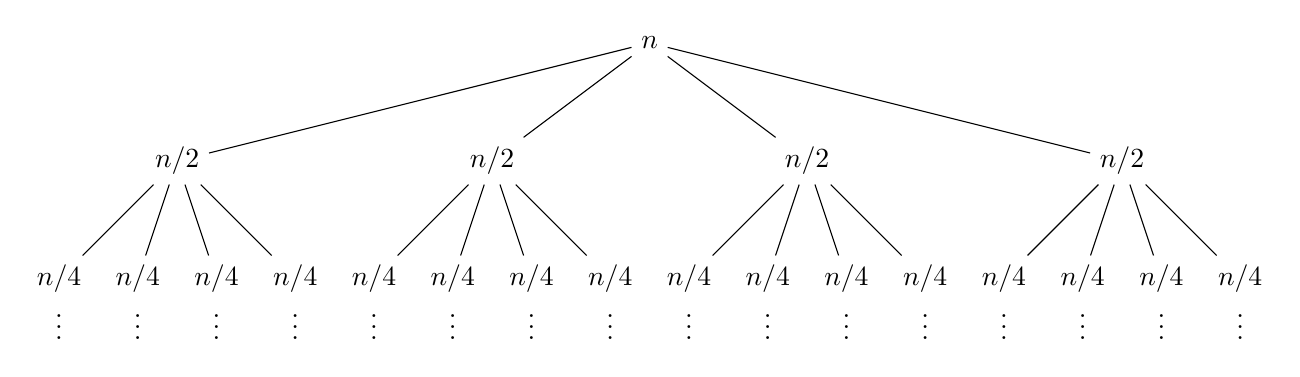
\begin{tikzpicture}[
    level distance=1.5cm,
    level 1/.style={sibling distance=4cm},
    level 2/.style={sibling distance=1cm},
    ]
    
    \node {$n$} % Root node
      child {node {$n/2$}
        child {node {$n/4$}
          child [level distance=0.25cm] {edge from parent[draw=none] child {node {$\vdots$} edge from parent[draw=none]}}
        }
        child {node {$n/4$}
          child [level distance=0.25cm] {edge from parent[draw=none] child {node {$\vdots$} edge from parent[draw=none]}}
        }
        child {node {$n/4$}
          child [level distance=0.25cm] {edge from parent[draw=none] child {node {$\vdots$} edge from parent[draw=none]}}
        }
        child {node {$n/4$}
          child [level distance=0.25cm] {edge from parent[draw=none] child {node {$\vdots$} edge from parent[draw=none]}}
        }
      }
      child {node {$n/2$}
        child {node {$n/4$}
          child [level distance=0.25cm] {edge from parent[draw=none] child {node {$\vdots$} edge from parent[draw=none]}}
        }
        child {node {$n/4$}
          child [level distance=0.25cm] {edge from parent[draw=none] child {node {$\vdots$} edge from parent[draw=none]}}
        }
        child {node {$n/4$}
          child [level distance=0.25cm] {edge from parent[draw=none] child {node {$\vdots$} edge from parent[draw=none]}}
        }
        child {node {$n/4$}
          child [level distance=0.25cm] {edge from parent[draw=none] child {node {$\vdots$} edge from parent[draw=none]}}
        }
      }
      child {node {$n/2$}
        child {node {$n/4$}
          child [level distance=0.25cm] {edge from parent[draw=none] child {node {$\vdots$} edge from parent[draw=none]}}
        }
        child {node {$n/4$}
          child [level distance=0.25cm] {edge from parent[draw=none] child {node {$\vdots$} edge from parent[draw=none]}}
        }
        child {node {$n/4$}
          child [level distance=0.25cm] {edge from parent[draw=none] child {node {$\vdots$} edge from parent[draw=none]}}
        }
        child {node {$n/4$}
          child [level distance=0.25cm] {edge from parent[draw=none] child {node {$\vdots$} edge from parent[draw=none]}}
        }
      }
      child {node {$n/2$}
        child {node {$n/4$}
          child [level distance=0.25cm] {edge from parent[draw=none] child {node {$\vdots$} edge from parent[draw=none]}}
        }
        child {node {$n/4$}
          child [level distance=0.25cm] {edge from parent[draw=none] child {node {$\vdots$} edge from parent[draw=none]}}
        }
        child {node {$n/4$}
          child [level distance=0.25cm] {edge from parent[draw=none] child {node {$\vdots$} edge from parent[draw=none]}}
        }
        child {node {$n/4$}
          child [level distance=0.25cm] {edge from parent[draw=none] child {node {$\vdots$} edge from parent[draw=none]}}
        }
      };
\end{tikzpicture}
\end{center}

\noindent \textbf{Time Analysis}: The first level takes $\tilde{O}(n^2)$ time. The second level takes $\tilde{O}\left(\frac{n^2}{2}\right)$ time. The third level takes $\tilde{O}\left(\frac{n^2}{4}\right)$ time. So the total time is $\tilde{O}(n^2)$. 

\noindent So, at level $i$:
\begin{itemize}
    \item There are $4^i$ edges.
    \item The work per edge $\leq (|\text{remaining vertices}|)^2 = \tilde{O}\left(\frac{n}{2^i}\right)^2 = \tilde{O}\left(\frac{n^2}{4^i}\right)$. 
\end{itemize}
This implies that the cost of the $i$th level is less than $\tilde O(n^2)$. Summing, we get a total cost $\tilde O(n^2)$.

Now we consider the probability that our algorithm succeeds. Again, we have a $4$-ary tree with a depth of $t = O(\log n)$. Each edge flips a coin where $P(\text{heads}) = \frac 14$. So what we want is a $t$ length chain of all heads. We can show the following result:
\begin{align*}
    P(\text{good path}) \geq \frac 1t \geq \Omega \left(\frac{1} {\log n}\right).
\end{align*}

The goal is an algorithm that succeeds with probability greater than $1 - \frac{1}{n^2}$. 

\noindent \textbf{Exercise:} $O(\log^2 n)$ repetitions suffice.



\end{document}